% !TEX program = pdflatex
\documentclass[12pt]{article}
 \usepackage[margin=1in]{geometry} 
\usepackage{amsmath,amsthm,amssymb,amsfonts, enumitem, fancyhdr, color, comment, graphicx, environ}
\pagestyle{fancy}
\setlength{\headheight}{65pt}
\newenvironment{problem}[2][Problem]{\begin{trivlist}
\item[\hskip \labelsep {\bfseries #1}\hskip \labelsep {\bfseries #2.}]}{\end{trivlist}}
\newenvironment{sol}
    {\emph{Solution:}
    }
    {
    \qed
    }
\specialcomment{com}{ \color{blue} \textbf{Comment:} }{\color{black}}
\NewEnviron{probscore}{\marginpar{ \color{blue} \tiny Problem Score: \BODY \color{black} }}
\usepackage[UTF8]{ctex}
\usepackage[version=4]{mhchem}
\lhead{Name: 陈稼霖\\ StudentID: 45875852}
\rhead{CHEM1111 \\ General Chemistry II \\ Spring 2019 \\ Homework 8}
\begin{document}
\begin{problem}{17.2}
Diagram the following galvanic cell, indicating the direction of flow of electrons in the external circuit and the motion of ions in the salt bridge.
\begin{center}
\ce{Ni(s)|Ni^{2+}(aq)||HCl(aq)|H2(g)|Pt(s)}
\end{center}
Write a balanced equation for the overall reaction in this cell.
\end{problem}
\begin{sol}
\begin{figure}[h]
\centering
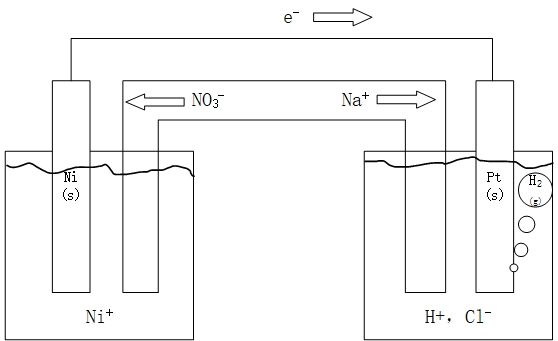
\includegraphics[scale=.8]{17_2.jpg}
\caption{Problem 17.2 Diagram of the galvanic cell}
\end{figure}
\\The balanced equation for the overall reaction in this cell is \ce{Ni(s) + 2H+(aq) -> Ni^{2+}(aq) + H2(g)}
\end{sol}

\begin{problem}{17.5}
A galvanic cell is constructed that has a zinc anode immersed in a \ce{Zn(NO3)2} solution and a platinum cathode immersed in an \ce{NaCl} solution equilibrated with \ce{Cl2(g)} at $1$ atm and $25^{\circ}$C. A salt bridge connects the two half-cells.\\
(a) Write a balanced equation for the cell reaction.\\
(b) A steady current of 0.800 A is observed to flow for a period of $25.0$ minutes. How much charge passes through the circuit during this time? How many moles of electrons is this charge equivalent to?\\
(c) Calculate the change in mass of the zinc electrode.\\
(d) Calculate the volume of gaseous chlorine generated or consumed as a result of the reaction.
\end{problem}
\begin{sol}
\\(a) The balanced equation for the cell reaction is \ce{Zn(s) + Cl2(g) -> Zn^{2+}(aq) + Cl-(aq)}\\
(b) The amount of charge passes through the circuit during this times is
\[
Q=it=0.800A\times(25.0\times60)s=\uline{1.20\times10^3C}
\]
The number of moles of electrons is
\[
n=\frac{Q}{F}=\frac{1.20\times10^3C}{96485.34C\cdot mol^{-1}}=\uline{0.0124mol}
\]
(c) Because the consumption of every mole of \ce{Zn} corresponds to transfer of $2$ mol electrons, the change in mass of the zinc electrode is
\[
m(Zn)=M(Zn)\frac{n}{2}=65.38g\cdot mol^{-1}\times\frac{0.0124mol}{2}=0.407g
\]
Therefore, the mass of zinc electrode \uline{decreased by $0.407$ g}.\\
(d) Because the consumption of every mole of gaseous chlorine corresponds to transfer of $2$ mol electrons, the volume of gaseous chlorine \uline{consumed} as a result of the reaction is
\[
V(Cl_2)=\frac{\frac{n}{2}RT}{P}=\frac{\frac{0.0124mol}{2}\times0.0821atm\cdot L\cdot mol^{-1}\cdot K^{-1}\times(25.0+273.15)K}{1atm}=\uline{0.152L}
\]
\end{sol}

\begin{problem}{17.11}
A \ce{Ni|Ni^{2+}||Ag+|Ag} galvanic cell is constructed in which the standard cell potential is 1.03 V. Calculate the free energy change at $25^{\circ}$C when $1.00$ g of silver plates out, if all concentrations remain at their standard value of $1$ \textsc{M} throughout the process. What is the maximum electrical work done by the cell on its surroundings during this experiment?
\end{problem}
\begin{sol}
The number of moles of \ce{Ag} plates out through out the process is
\[
n(Ag)=\frac{m(Ag)}{M(Ag)}=\frac{1.00g}{107.87g\cdot mol^{-1}}=9.27\times10^{-3}mol
\]
Because the generation of every mole of \ce{Ag} corresponds to transfer of $1$ mol electrons, the number of moles of electron transfered through out the process is
\[
n=n(Ag)=9.27\times10^{-3}mol
\]
The change of the free energy change through out the process is
\[
\Delta G^{\circ}=-nFE_{cell}^{\circ}=-9.27\times10^{-3}mol\times96485C\cdot mol^{-1}\times1.03V=\uline{-921J}
\]
Because $w_{elec}=\Delta G^{\circ}$, the maximum electrical work done by the cell on its surrounding during this experiment is \uline{$921$ J}.
\end{sol}

\begin{problem}{17.25}
The following reduction potentials are measured at pH 0:
\begin{center}
\ce{BrO3^- + 6H3O+ + 5e- -> \frac{1}{2}Br2(l) + 9H2O}~~$E^{\circ}=1.52V$\\
\ce{Br2(l) + 2e- -> 2Br-}~~$E^{\circ}=1.065V$
\end{center}
(a) Will bromine disproportionate spontaneously in acidic solution?\\
(b) Which is the stronger reducing agent at pH $0$: \ce{Br2(l)} or \ce{Br-}?
\end{problem}
\begin{sol}
\\(a) The equation of the disproportionation reaction of bromine in acidic solution and its standard cell potential is
\begin{center}
\ce{3Br2(l) + 9H2O -> 5Br- + BrO3^- + 6H3O+}~~$E^{\circ}=-0.455V$
\end{center}
The change of free energy change during the disproportionation reaction of bromine is positive
\[
\Delta G^{\circ}=-nFE^{\circ}>0
\]
Therefore, bromine \uline{will not} disproportionate in acidic solution.\\
(b) Because the standard potential of the reaction \ce{Br2(l) + 2e- -> 2Br-} is positive, its change of free energy is negative, which means it can proceed spontaneously. In this reaction, \ce{Br2(l)} is reduced to \ce{Br-}. Therefore, \uline{\ce{Br-} is the stronger reducing agent}.
\end{sol}

\begin{problem}{17.26}
The following reduction potentials are measured at pH $14$:
\begin{center}
\ce{ClO- + H2O + 2e- -> Cl- + 2OH-}~~$E^{\circ}=0.90V$\\
\ce{ClO2^- + H2O + 2e- -> ClO- + 2HO-}~~$E^{\circ}=0.59V$
\end{center}
(a) Will \ce{ClO-} disproportionate spontaneously in basic solution?\\
(b) Which is the stronger reducing agent at pH $14$: \ce{ClO-} or \ce{Cl-}?
\end{problem}
\begin{sol}
\\(a) The equation of the disproportionation reaction of \ce{ClO-} in basic solution and its standard cell potential is
\begin{center}
\ce{2ClO- -> Cl- + ClO2^-}~~$E^{\circ}=0.31V$
\end{center}
The change of free energy change during the disproportionation reaction of bromine is negative
\[
\Delta G^{\circ}=-nFE^{\circ}>0
\]
Therefore, bromine \uline{will} disproportionate in acidic solution.\\
(b) Because the standard potential of the reaction \ce{ClO- + H2O + 2e- -> Cl- + 2OH-} is positive, its change of free energy is negative, which means it can proceed spontaneously. In this reaction, \ce{ClO-} is reduced to \ce{Cl-}. Therefore, \uline{\ce{Cl-} is the stronger reducing agent}.
\end{sol}
\end{document}